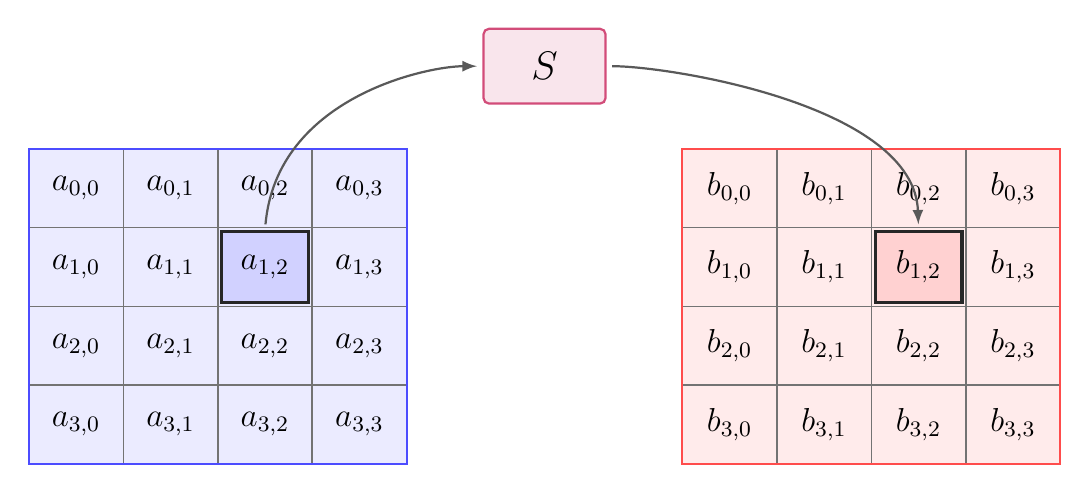
\begin{tikzpicture}[>=latex]

% --- Global TikZ Styles ---
\tikzset{
    matrixA/.style={
        fill=blue!8
    },
    matrixB/.style={
        fill=red!8
    },
    frameA/.style={
        draw=blue!70,
        thick
    },
    frameB/.style={
        draw=red!70,
        thick
    },
    operatorbox/.style={
        fill=purple!10,
        draw=purple!70,
        thick,
        rounded corners=2pt,
        minimum width=1.55cm,
        minimum height=0.95cm,
        font=\Large
    },
    gridline/.style={
        draw=black!55,
        line width=0.55pt
    },
    highlightA/.style={
        fill=blue!18,
        draw=black!85,
        very thick,
        minimum width=1.10cm,
        minimum height=0.90cm,
        inner sep=0pt
    },
    highlightB/.style={
        fill=red!18,
        draw=black!85,
        very thick,
        minimum width=1.10cm,
        minimum height=0.90cm,
        inner sep=0pt
    },
    arrow/.style={
        ->,
        >=latex,
        thick,
        draw=black!65,
        shorten >=2pt,
        shorten <=2pt
    },
    element/.style={
        font=\large
    }
}

% ==================================================
% --- Left array A ---
% ==================================================

\begin{scope}[shift={(-4.8,-1.8)}]

    % Background
    \path[matrixA] (0,0) rectangle (4.8,4);

    % Grid
    \draw[gridline]
        (0,0) grid[xstep=1.2,ystep=1] (4.8,4);

    % Colored outer frame
    \draw[frameA] (0,0) rectangle (4.8,4);

    % Highlight a_{1,2}
    \node[highlightA] (a12) at (3.0,2.5) {};

    % Matrix entries a_{i,j}
    \foreach \i in {0,...,3}{
        \foreach \j in {0,...,3}{
            \node[element]
                at ({0.6+1.2*\j},{3.5-\i})
                {$a_{\i,\j}$};
        }
    }

\end{scope}

% ==================================================
% --- Right array B ---
% ==================================================

\begin{scope}[shift={(3.5,-1.8)}]

    % Background
    \path[matrixB] (0,0) rectangle (4.8,4);

    % Grid
    \draw[gridline]
        (0,0) grid[xstep=1.2,ystep=1] (4.8,4);

    % Colored outer frame
    \draw[frameB] (0,0) rectangle (4.8,4);

    % Highlight b_{1,2}
    \node[highlightB] (b12) at (3.0,2.5) {};

    % Matrix entries b_{i,j}
    \foreach \i in {0,...,3}{
        \foreach \j in {0,...,3}{
            \node[element]
                at ({0.6+1.2*\j},{3.5-\i})
                {$b_{\i,\j}$};
        }
    }

\end{scope}

% ==================================================
% --- Operator S ---
% ==================================================

\node[operatorbox] (S) at (1.75,3.25) {$S$};

% ==================================================
% --- Curved arrows ---
% ==================================================

% From a_{1,2} to S
\draw[arrow]
    (a12.north)
    .. controls (-1.65,2.85) and (0.25,3.25) ..
    (S.west);

% From S to b_{1,2}
\draw[arrow]
    (S.east)
    .. controls (3.35,3.25) and (6.45,2.75) ..
    (b12.north);

\end{tikzpicture}